
%%%----------------------------------------------------------
\chapter{Summary}
%%%----------------------------------------------------------
%Give a concise (and honest) summary of what has been accomplished and what not. 
%Point out issues that may warrant further investigation.

This project is a partial implementation of the article described in \cite{Zhang2009}, using the \Numpy{} module and the \OpenCV{} python bindings. 
The reader should look at \cref{sec:implemented components} if a more in-depth understanding of which components of the original article were implemented.
A comparison between a depth-map obtained by Zhang (left) and one estimated using the provided implementation(right) can be seen in \cref{fig:disp_comparison}.

\begin{figure}[!h]
	\centering
	\begin{minipage}[c]{.45\textwidth}
		\centering
		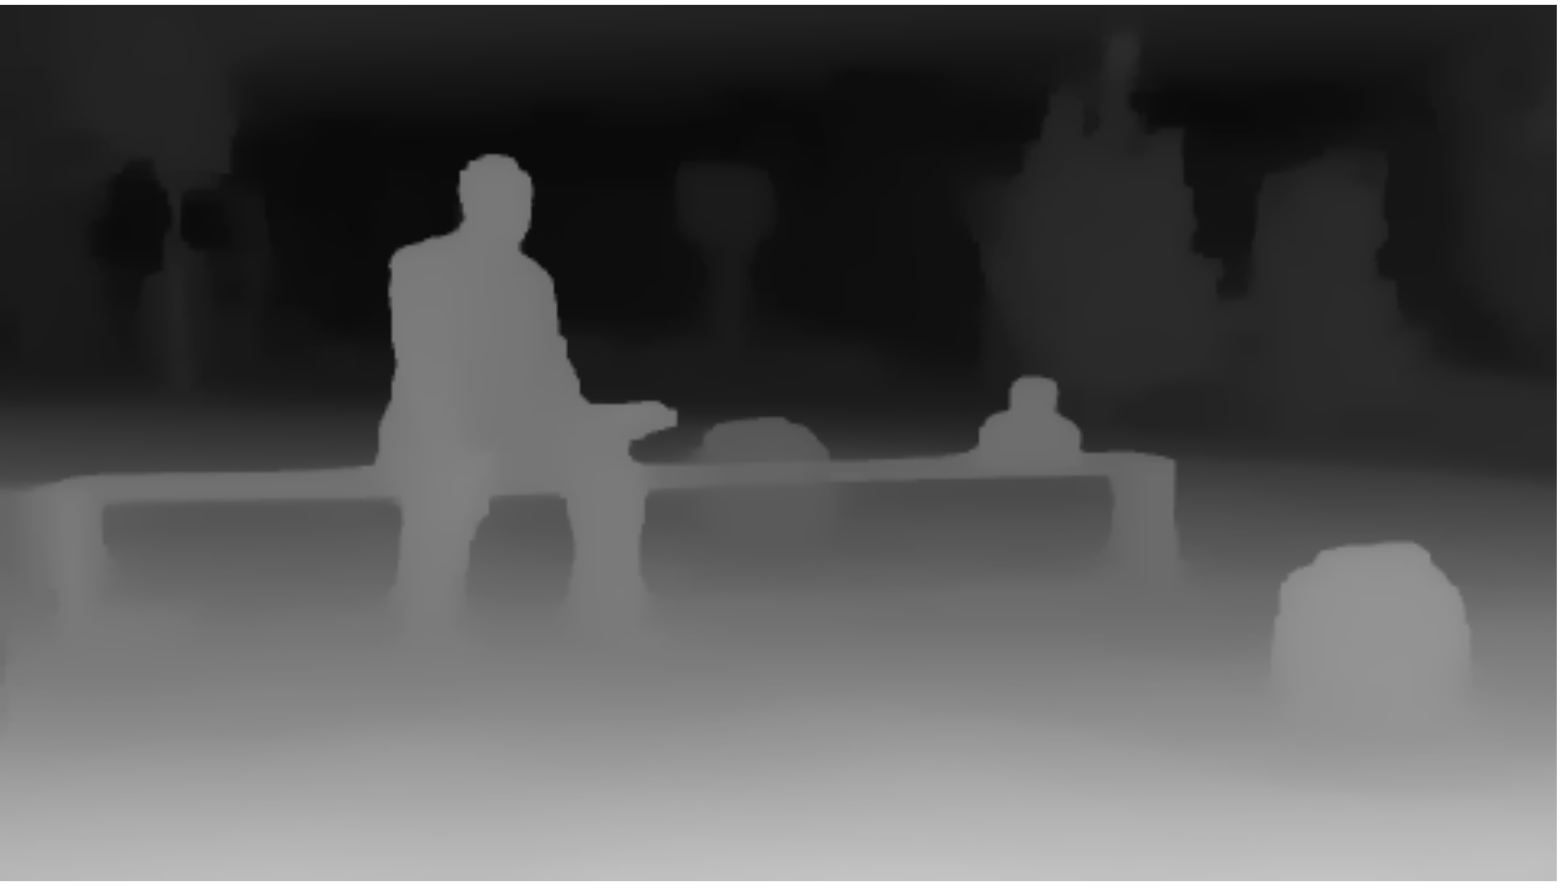
\includegraphics[width=\textwidth]{summary/depthmap_zhang.png}
		%\caption{Caption for image}
	\end{minipage}
	\begin{minipage}[c]{.45\textwidth}
		\centering
		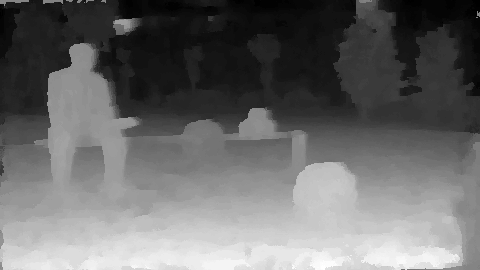
\includegraphics[width=\textwidth]{summary/depthmap_giorgio.png}
		%\caption{Caption for image}
	\end{minipage}
\caption{Comparison between depth-maps estimated using the complete original implementation (left) and depth-maps estimated using the partial implementation provided.}\label{fig:disp_comparison}
\end{figure}

\subsection{Future Work}
A simple improvement over the project could be the implementation of the remaining components. A further expansion to the project could also be the introduction of hardware specific accelerated libraries, such as \Cupy{} or \Pytorch.
